\usetikzlibrary{angles,quotes}
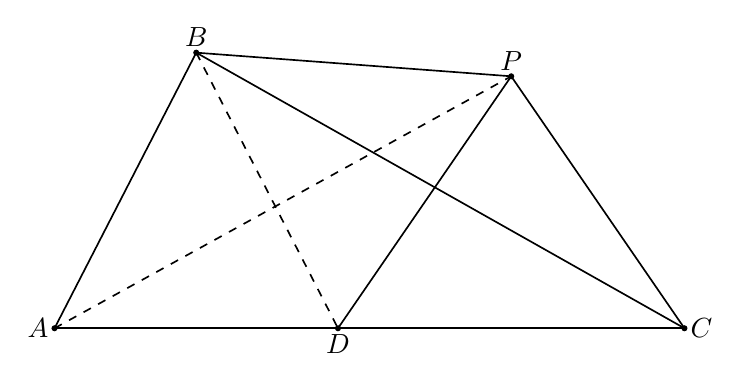
\begin{tikzpicture}[x=1cm,y=1cm,font=\normalsize,
  geometry edge/.style={solid,line width=.6pt},
  geometry label/.style={font=\normalsize,inner sep=0pt}]
\coordinate (A) at (0,0);
\coordinate (C) at (8,0);
\coordinate (D) at (3.6,0);
\coordinate (B) at (1.8,3.5);
\coordinate (P) at (5.8,3.2);
\draw[geometry edge] (A)--(B);
\draw[geometry edge] (B)--(P);
\draw[geometry edge] (P)--(C);
\draw[geometry edge] (A)--(C);
\draw[geometry edge] (P)--(D);
\draw[geometry edge] (B)--(C);
\draw[geometry edge,dashed] (A)--(P);
\draw[geometry edge,dashed] (B)--(D);
\fill (A) circle (1.1pt) (B) circle (1.1pt) (C) circle (1.1pt) (D) circle (1.1pt) (P) circle (1.1pt);
\node[geometry label,anchor=east] at ([xshift=-2pt]A) {$A$};
\node[geometry label,anchor=south] at ([yshift=2pt]B) {$B$};
\node[geometry label,anchor=south] at ([yshift=2pt]P) {$P$};
\node[geometry label,anchor=west] at ([xshift=2pt]C) {$C$};
\node[geometry label,anchor=north] at ([yshift=-2pt]D) {$D$};
\end{tikzpicture}
